\documentclass[11pt]{article}

\usepackage{tikz}
\usepackage{tikz-qtree}
\usetikzlibrary{trees}
\usetikzlibrary{automata, arrows.meta, positioning, shapes.geometric}

\usepackage{xcolor}
\usepackage[margin=1.0in]{geometry}
\usepackage{amsfonts,amsmath,amssymb}

\tikzset{every tree node/.style={minimum width=2em,draw,circle},
         blank/.style={draw=none},
         edge from parent/.style=
         {draw,edge from parent path={(\tikzparentnode) -- (\tikzchildnode)}},
         level distance=2.5em}

\begin{document}
\begin{flushleft}

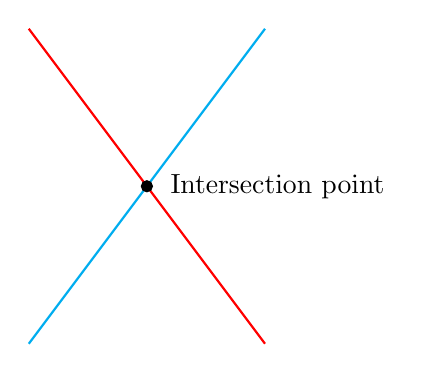
\begin{tikzpicture}
\draw[red, thick] (-1,2) -- (2,-2);
\draw[cyan, thick] (-1,-2) -- (2,2);
\filldraw[black] (0.5,0) circle (2pt) node[anchor=west]{\hspace{0.5em}Intersection point};
\end{tikzpicture}

\vspace{1em}

\begin{tikzpicture}
\draw (-2,0) -- (2,0);
\filldraw [gray] (0,0) circle (2pt);
\draw (-2,-2) .. controls (0,0) .. (2,-2);
\draw (-2,2) .. controls (-1,0) and (1,0) .. (2,2);
\end{tikzpicture}

\vspace{1em}

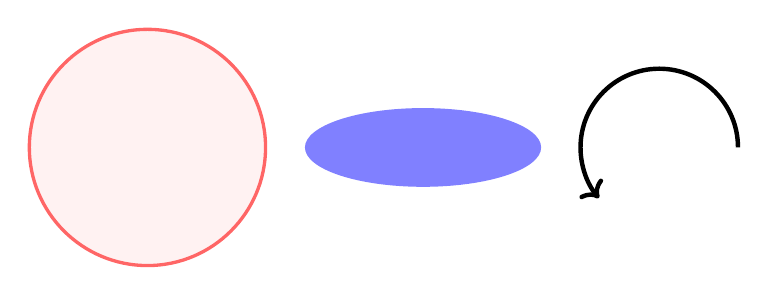
\begin{tikzpicture}
\filldraw[color=red!60, fill=red!5, very thick](-1,0) circle (1.5);
\fill[blue!50] (2.5,0) ellipse (1.5 and 0.5);
\draw[ultra thick, ->] (6.5,0) arc (0:220:1);
\end{tikzpicture}

\newpage
%%%%% Automata %%%%%
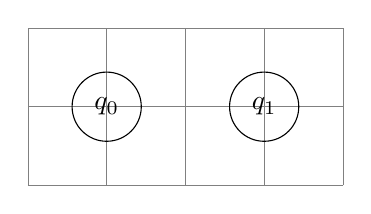
\begin{tikzpicture}
% Help grid
    \draw [help lines] (3,-1) grid (-1,1);
% State 1
    \node [state] {$q_0$};
% State 2
    \node [state] at (2,0) {$q_1$};
\end{tikzpicture}

\newpage
%%%%% Binary Trees %%%%%
\textbf{Binary Trees}
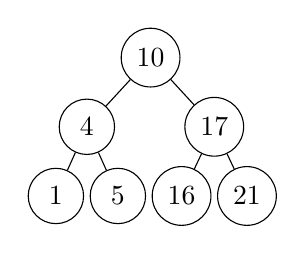
\begin{tikzpicture}
\Tree
[.10 
    [.4 
        [.1 ]
        [.5 ]    
    ]
    [.17
        [.16 ]
        [.21 ]
    ]
]
\end{tikzpicture}\\ \vspace{0.5em}

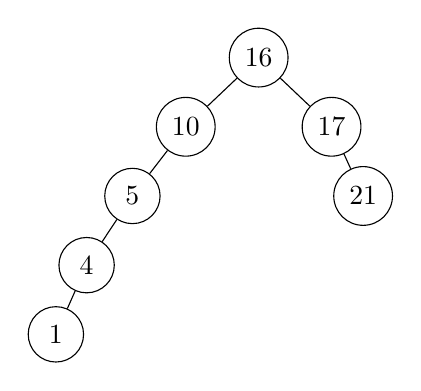
\begin{tikzpicture}
\Tree
[.16
    [.10 
        [.5
            [.4
                [.1 ]
                \edge[blank]; \node[blank]{};
            ]
            \edge[blank]; \node[blank]{};
        ]
        \edge[blank]; \node[blank]{};
    ]
    [.17 
        \edge[blank]; \node[blank]{};
        [.21 ]
    ]
]
\end{tikzpicture}\\ \vspace{0.5em}

\end{flushleft}
\end{document}